% % \documentclass[12pt]{article}%


% \documentclass[10pt,nofootinbib,floatfix,superscriptaddress]{revtex4} % ,preprint ,endfloats,floatfix,titlepage,endfloats,
% %\documentclass[12pt,a4paper,final]{iopart}
% % \documentclass[nofootinbib,floatfix,reprint,prl,endfloats,superscriptaddress]{revtex4} %  ,floatfix
% %\usepackage{natbib}

% \usepackage[utf8]{inputenc}
% \usepackage{nima,graphicx,amsmath,amssymb,color}%,hyperref}
% \usepackage{mathrsfs}
% %\usepackage{graphicx}
% \usepackage{comment}
% % \newcommand{\Ls}{\mathscr{L}}

% % \usepackage{setspace}
% % \linespread{1.5}

% \newcommand{\lrto}{\leftrightarrow}
% % \marginparwidth 0pt
% % \oddsidemargin  0pt
% % \evensidemargin  0pt
% % \marginparsep 0pt
% % \topmargin   -0.25in 
% % \textwidth   6.5in
% %\textheight  9.0in
% \newcommand{\RNum}[1]{\uppercase\expandafter{\romannumeral #1\relax}}
% \newcommand{\outNim}[1]{}
% %
% % \documentclass{article}
% \usepackage{array}

% \begin{document}
% %\centerline{\Huge Phases of Physical 3D Networks}

% \title{Phases of Physical 3D Networks}
% \author{Nima Dehmamy\thanks{nidami@gmail.com}}
% \affiliation{Center for Complex Network Research, Northeastern University, Boston, USA}
% \author{Soodabeh Milanlouei}
% \affiliation{Center for Complex Network Research, Northeastern University, Boston, USA}
% \author{Albert-L\'aszl\'o Barab\'asi}
% \affiliation{Center for Complex Network Research, Northeastern University, Boston, USA}
% \affiliation{Center for Cancer Systems Biology, Dana Farber Cancer Institute, Boston, USA}
% \affiliation{Department of Medicine, Brigham and Women’s Hospital, Harvard Medical School, Boston, USA}
% \affiliation{Center for Network Science, Central European University, Budapest, Hungary}
% %\maketitle
% \date{\today}
% \maketitle
\documentclass[10pt]{article}%
% \documentclass[nofootinbib,preprint,floatfix,endfloats]{revtex4} % ,endfloats,floatfix
%\documentclass[12pt,a4paper,final]{iopart}

\usepackage[utf8]{inputenc}
\usepackage{nima,graphicx,amsmath,amssymb,color}%,hyperref}
\usepackage{mathrsfs}
%\usepackage{graphicx}
\usepackage{comment}
\usepackage{setspace}
% \newcommand{\Ls}{\mathscr{L}}

% \newcommand{\lrto}{\leftrightarrow}
 \marginparwidth 0pt
 \oddsidemargin  0pt
 \evensidemargin  0pt
 \marginparsep 0pt
 \topmargin   -1.25in 
\textwidth   6.5in
 \textheight  10.0 in
\newcommand{\RNum}[1]{\uppercase\expandafter{\romannumeral #1\relax}}
\newcommand{\outNim}[1]{}
%

\begin{document}
\title{Structural Phase Transition in Physical Networks Embedded in 3D}
\author{Nima Dehmamy\thanks{nidami@gmail.com}, Soodabeh Milanlouei, Albert-L\'aszl\'o Barab\'asi \\
{\em CCNR, Northeastern University, Boston, 02115 MA} }
% \date{\today}
\maketitle
\outNim{
\medskip
\centerline{Nima Dehmamy\footnote{nidami@gmail.com}, Soodabeh Milanlouei, Albert-L\'aszl\'o Barab\'asi}
\centerline{\today}
\bigskip
}
 % \begin{abstract}
% \begin{document}
{%\bf 
In many physical networks, from neurons in brain \cite{kasthuri2015saturated,oh2014mesoscale} to bundles of cables carrying power in infrastructural systems or underground hyphal networks \cite{friese1991spread}, the nodes and links are physical objects unable to cross each other.
These non-crossing conditions constrain their layout and limit how these networks form, evolve and function. 
Despite the recent development of an extensive theoretical framework to describe the structure and evolution of real networks, none of the currently existing network models take into account this physicality. 
Furthermore, the  network layout algorithms currently in use are variants of the Force-Directed Layout (FDL) algorithm \cite{kamada1989algorithm,fruchterman1991graph}, which also assumes dimensionless nodes and links, being inherently incapable of visualizing densely packed physical networks, like neurons in the brain.
Here, we develop a modeling framework inspired by manifold dynamics that accounts for the physical reality of nodes and links, allowing us to 
understand how the non-crossing conditions affect the network layout and characteristics. 
We find that for small link thicknesses, $r_L$, the layout is largely independent of $r_L$. 
In this weakly interacting phase, while there are numerous potential crossings, the layout avoids conflicts via local link rearrangements, without the need to alter the overall geometry of the layout. 
Once $r_L$ reaches a critical threshold, we observe the emergence of a strongly interacting phase, where multiple geometric quantities, from total link length to link curvature, scale with $r_L$. 
We show that this transition is now driven by excluded volume interactions, a finding that allows us to analytically derive the transition point.
We also
and document a deep universality, finding that the scaling law characteristics of the layout geometry are largely independent of the underlying network topology. 
Finally, we find that networks display a solid-like response to stress in the weakly interacting phase, whereas they behave in a gel-like fashion in the strongly interacting phase, indicating that the observed layout transition  affects the physical properties of the network. 
These findings not only unveil the fundamental geometrical constraints obeyed by physical networks, but have direct application for 3D printing of realistic networks and for the layout of densely packed mammalian brains.
} 
%\end{abstract}
%\maketitle
%\end{document}
%\newpage
\begin{figure}
\centering
%\vspace{-2cm}
%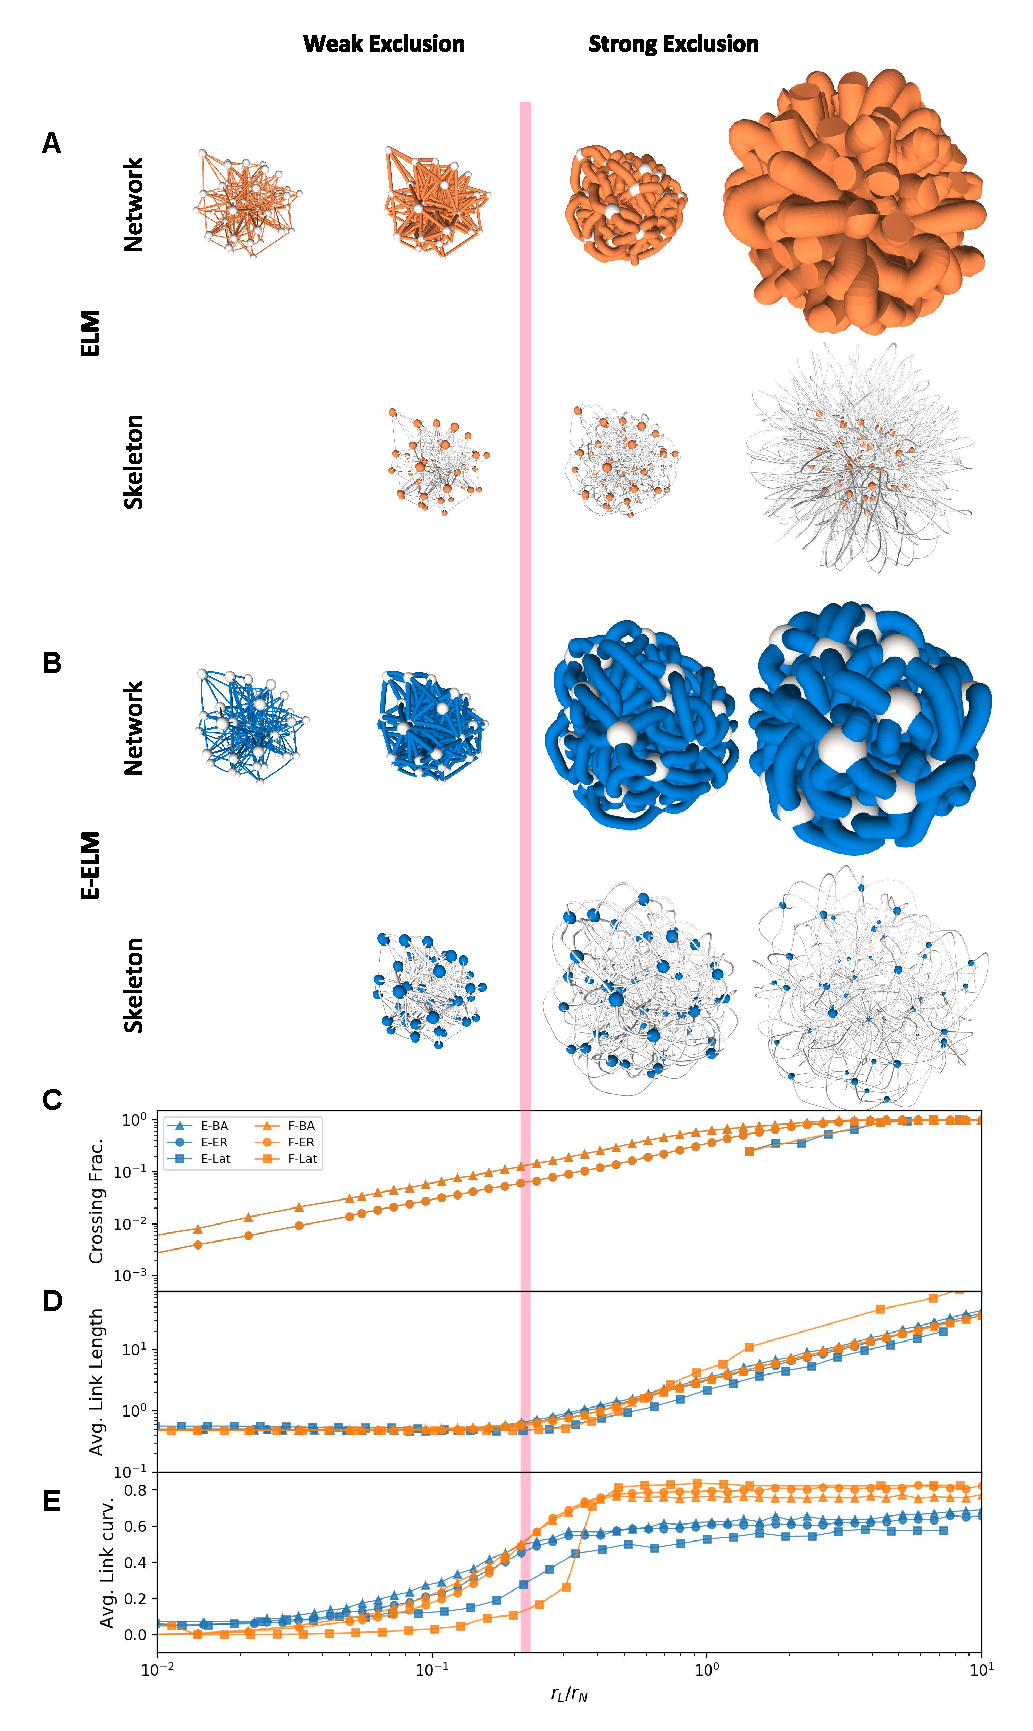
\includegraphics[width=.69\columnwidth]{fig-09-19/phase-051817.pdf}
% 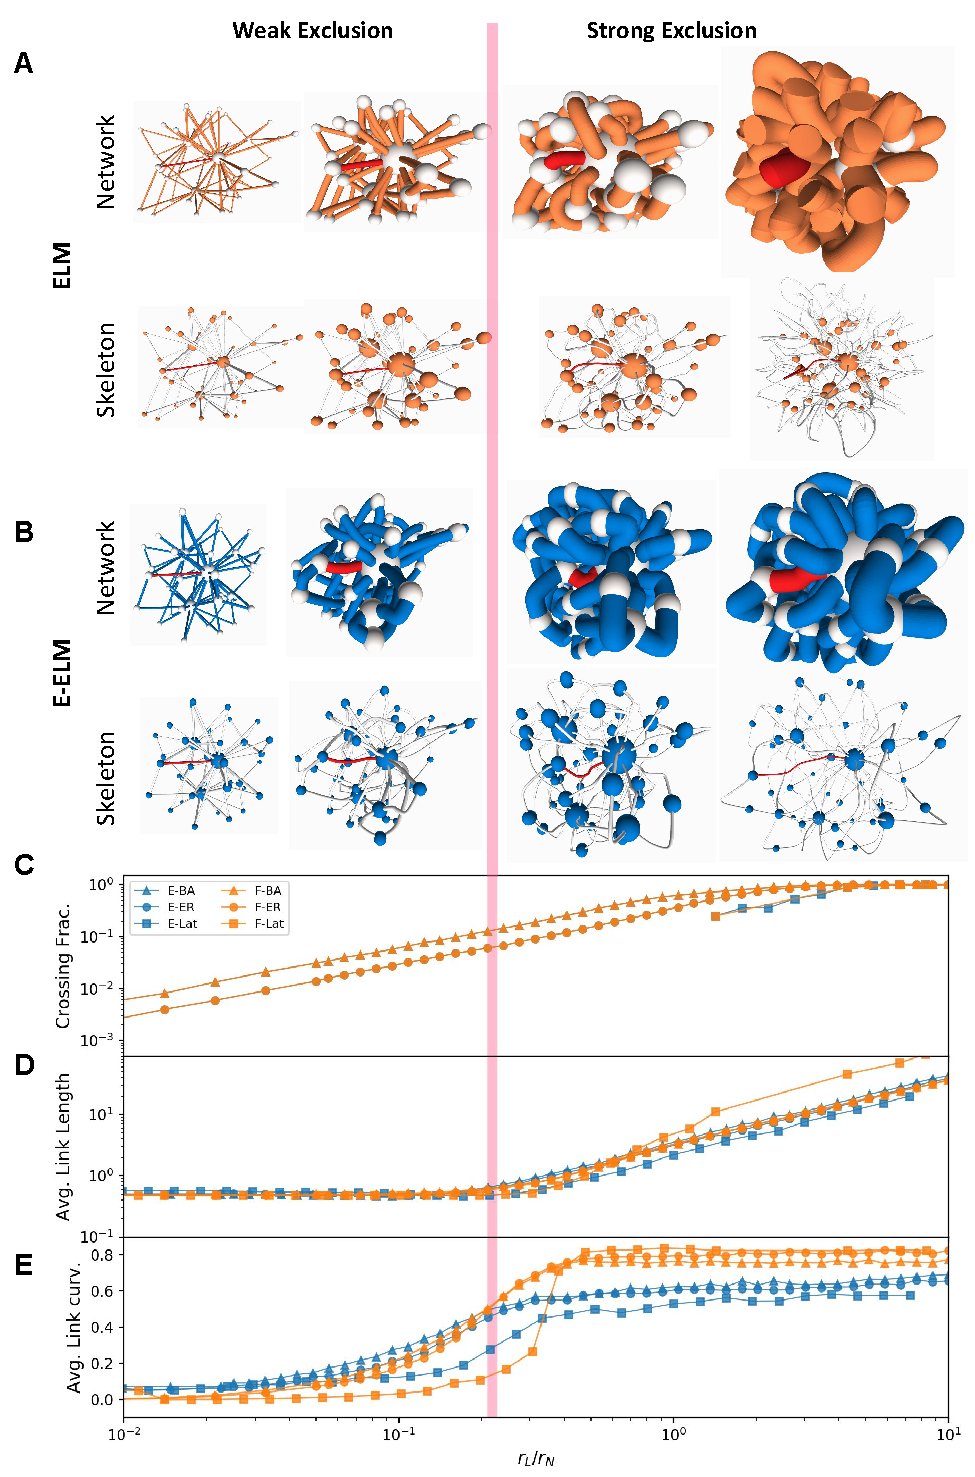
\includegraphics[width=.69\columnwidth]{fig-09-19/phase-061717.pdf}
% 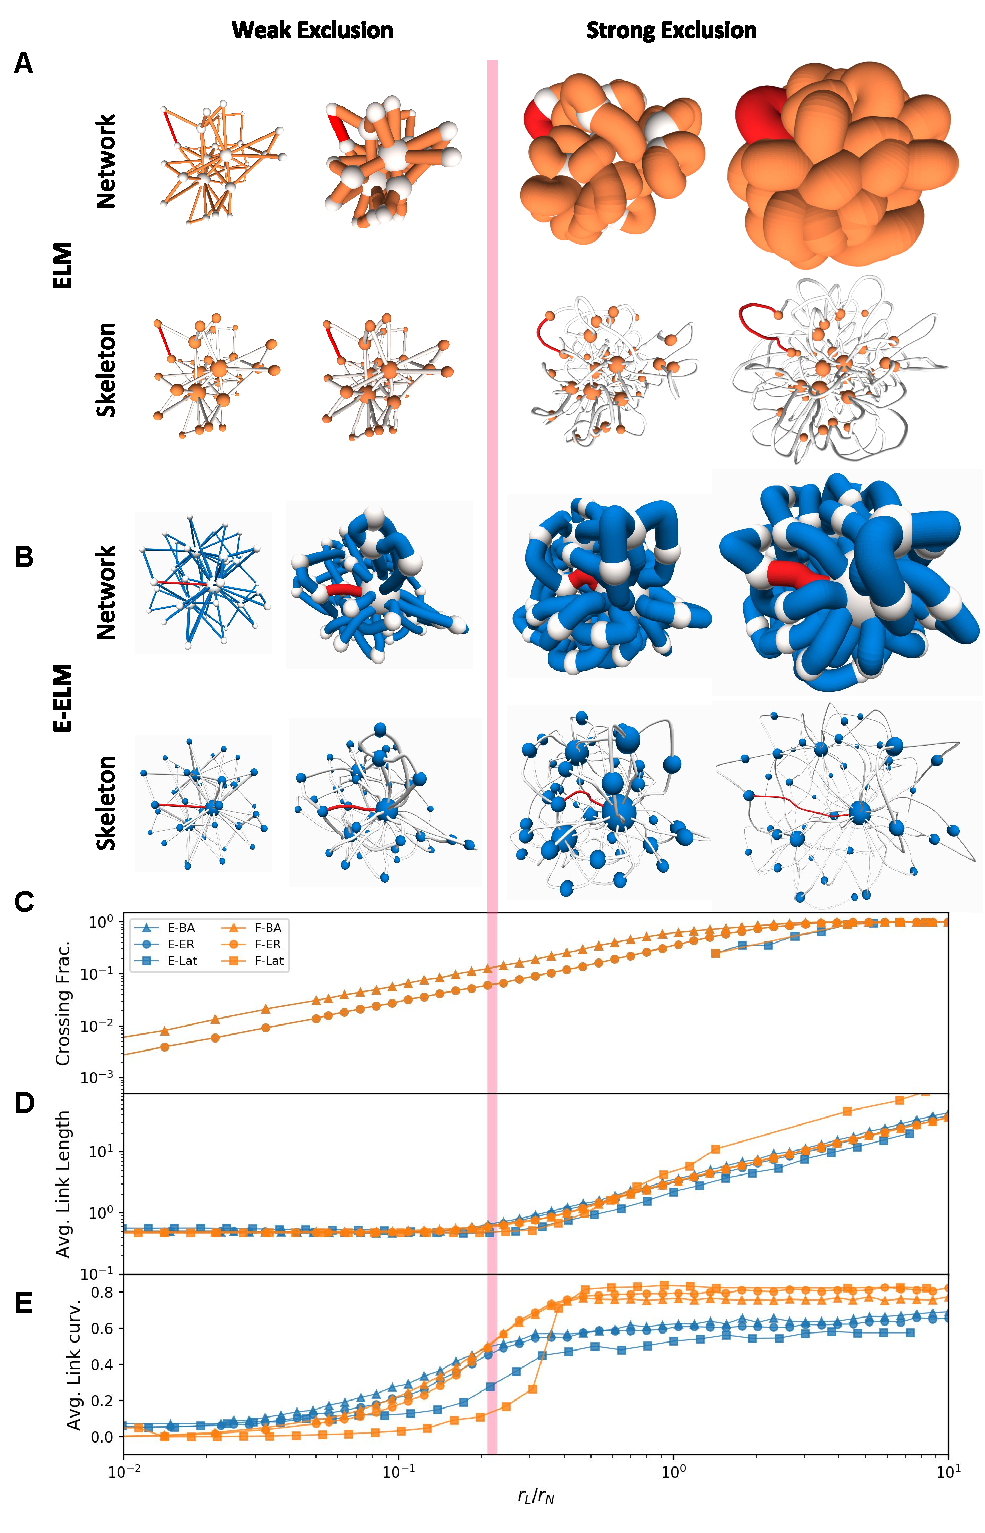
\includegraphics[width=.69\columnwidth]{fig-09-19/phase-071517.pdf}
% 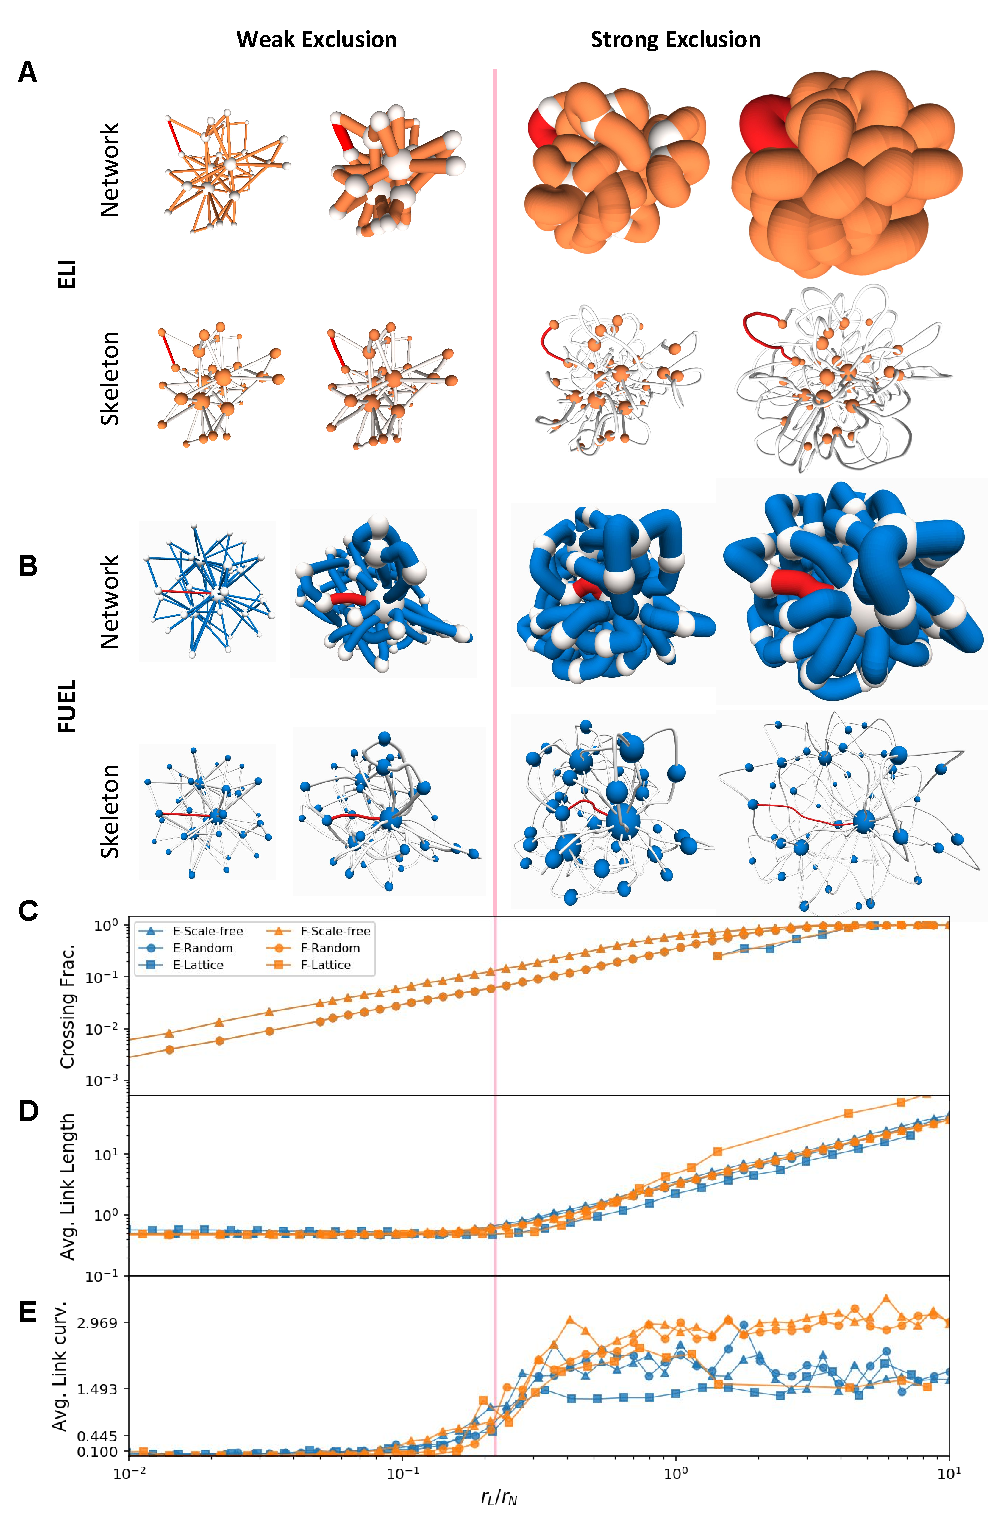
\includegraphics[width=.69\columnwidth]{fig-09-19/phase-full-071917.pdf}
%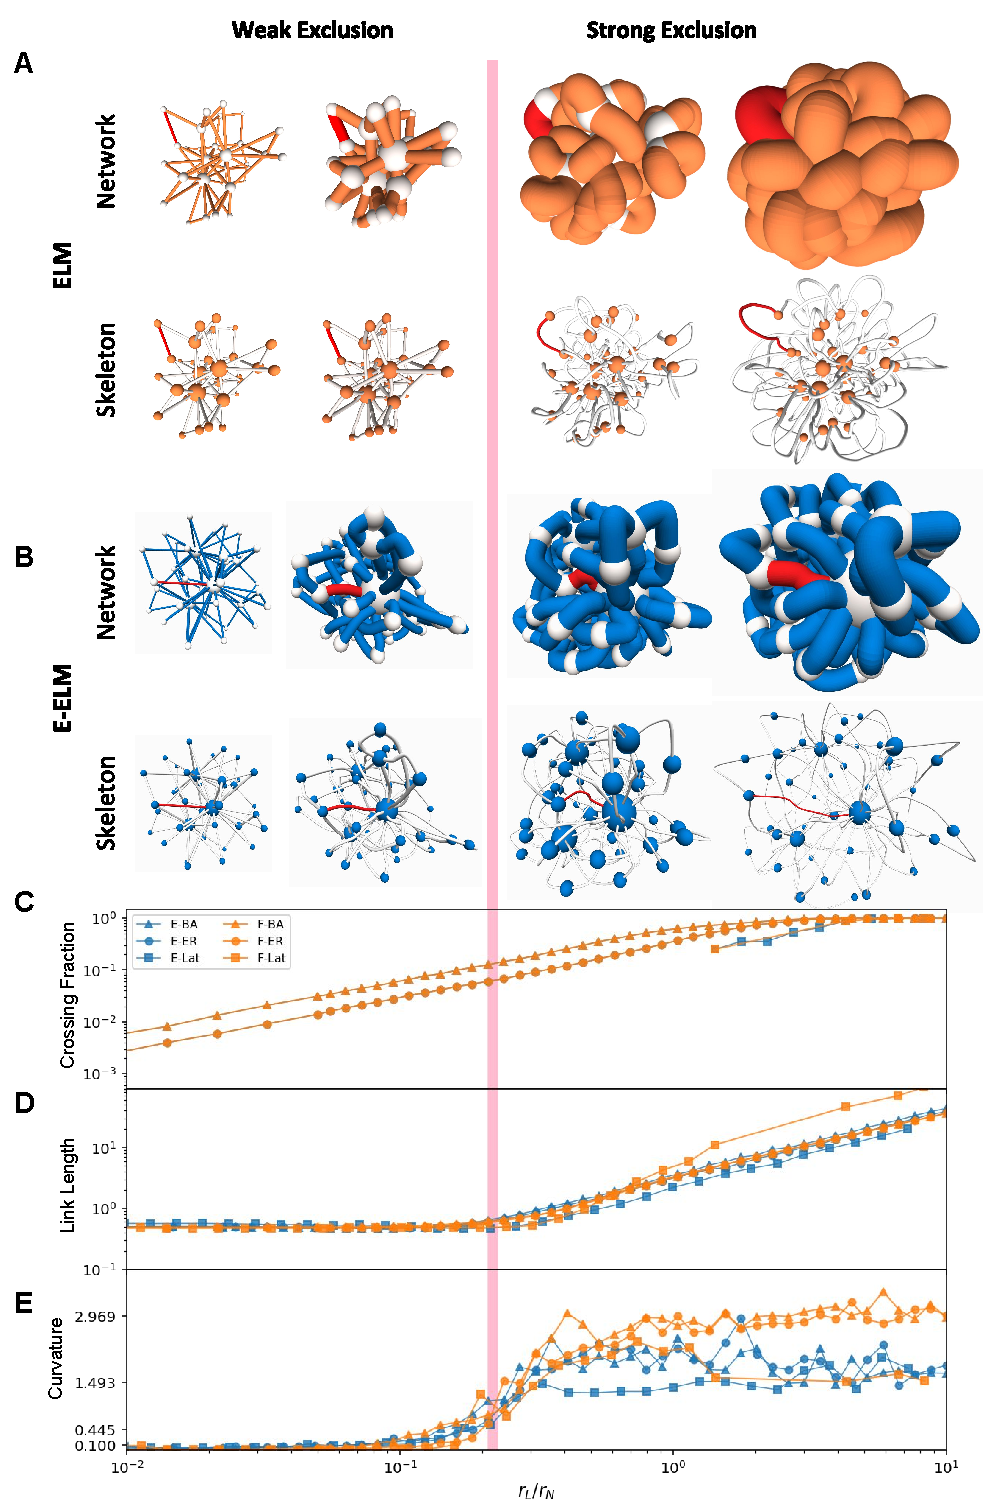
\includegraphics[width=.69\columnwidth]{fig-09-19/3D-phase.pdf}
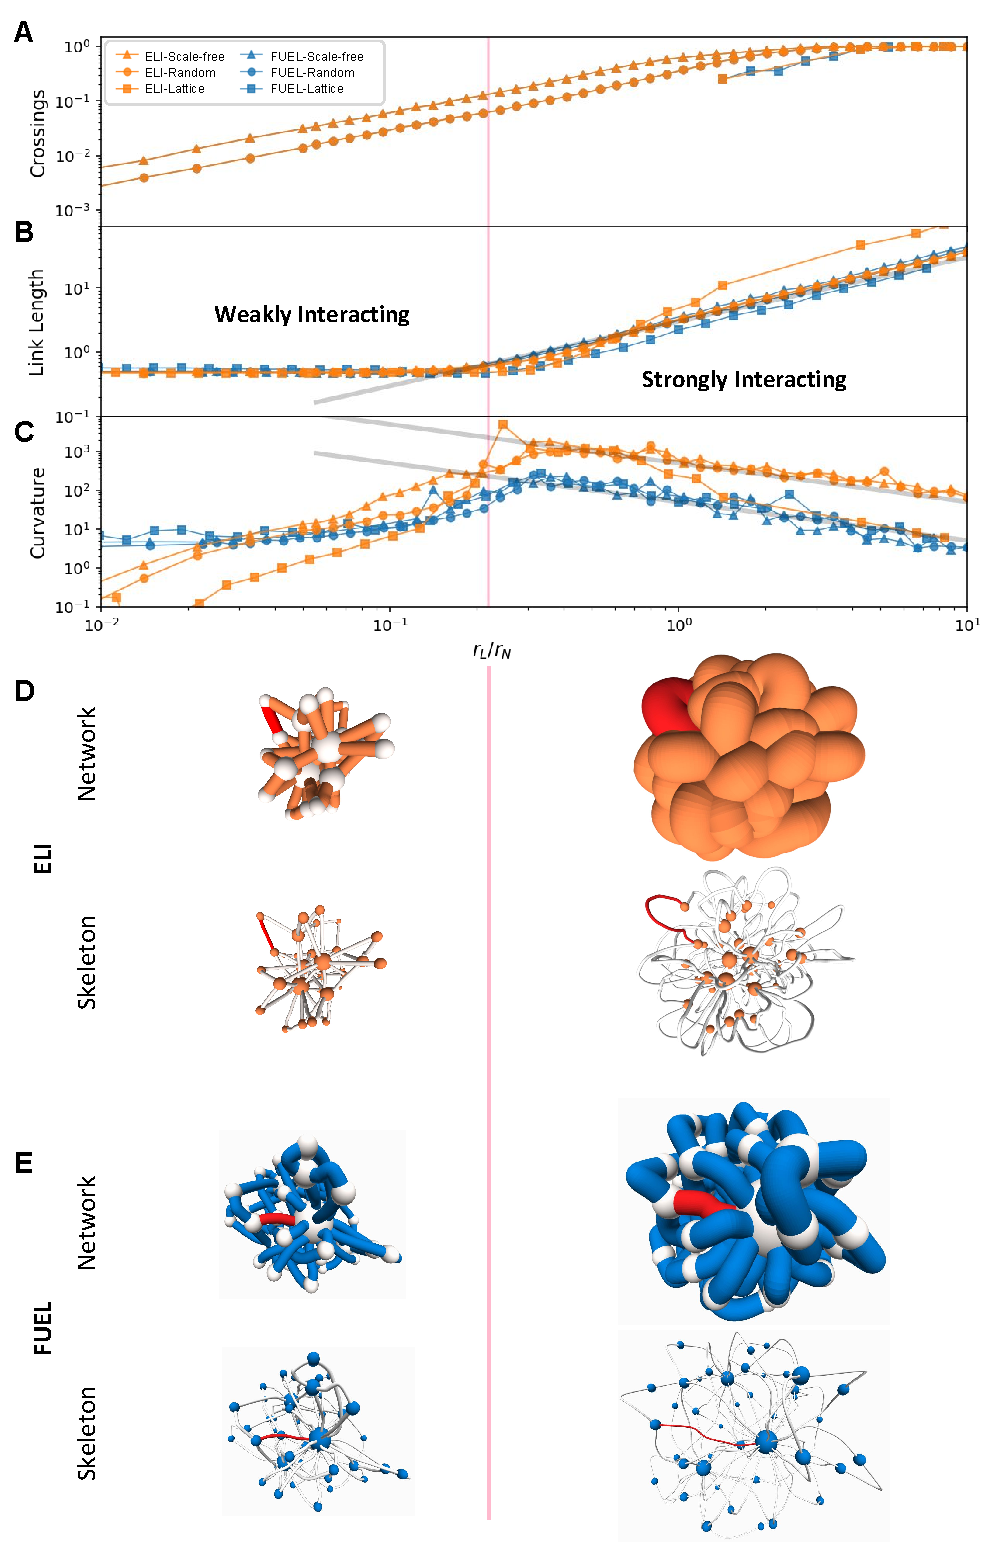
\includegraphics[width=.69\columnwidth]{fig-09-19/3D-phase-compare-092617.pdf}
\caption{%3D layouts  using ELM and E-ELM, and their phase diagram.
         \scriptsize {\bf Phases of ELI vs. FUEL:} {\bf (A)} 
         Orange lines correspond to ELI and blue lines to FUEL.
         For each we show three network topologies: Scale-free, Random and Lattice.
         %Each symbol signifies a network topology: ER: Erdős-Renyi; BA: Barabasi-Albert; Lat: the 3D regular lattice.
         ({\bf B}) The average link length remains more or less constant in the weakly interacting regime (small $r_L/r_N$), but grows linearly in the strongly interacting regime for all three topologies and for both ELI and FUEL, unable to distinguish between topologies.  
         ({\bf C}) While total Link curvature, normalized by the average link length $\be{l}$, of BA and ER overlap almost completely in both ELI and FUEL (bottom), the lattice does differ from them in the ELI.
         {\bf ELI and FUEL geometries:} 
         ELI ({\bf D}, orange) and FUEL ({\bf E}, blue) used on a BA $N=10, m=3$. 
         Below each layout we show the skeleton, where the links are made thin, to show the paths of the links.
         ELI layouts were generated using the double-ellipsoidal metric, instead of Euclidean distance, to avoid links bending onto themselves in the strongly interacting phase. 
         At small thicknesses, $r_L \ll r_N$, both layouts are the similar to FDL. At larger $r_L$ in ELI links start bending to avoid each other. 
         At very large $r_L$, links don't fit inside the region containing the nodes and start making outward arcs. 
         FUEL at large $r_L$ behaves more gently and the layout size just grows linearly with the $r$.
         One link is highlighted as red to contrast the variation in link trajectories with increasing link thickness.
         The gray line in {\bf B} shows linear increase with $r_L$ and the gray lines in {\bf C} show a $1/r_L$ trend. 
          }    
    \label{fig:phase-compare}
\end{figure}

\bibliographystyle{abbrv}
\bibliography{mybib}
\end{document}


